\documentclass[varwidth=true, border=2pt]{standalone}

\usepackage{pgfplots}
\usepackage{tikz}

\usetikzlibrary{calc,patterns,angles,quotes}

\begin{document}
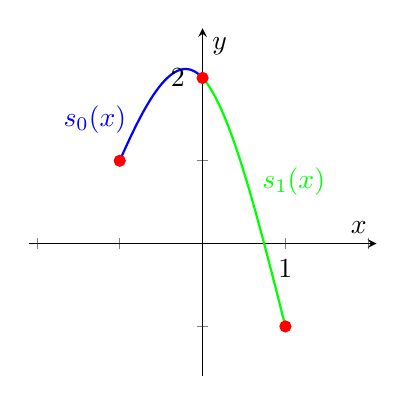
\begin{tikzpicture}
    \begin{axis}[
        legend pos=south east,
        axis x line=middle,
        axis y line=middle,
  %    axis line style={draw=none},
  %    tick style={draw=none},
	xticklabels=\empty,
	yticklabels=\empty
        grid = none ,
        width=6cm,
        height=6cm,
        grid style={dashed, gray!1},
        xmin=-1.75,     % start the diagram at this x-coordinate
        xmax= 1.75,    % end   the diagram at this x-coordinate
        ymin=-1.25,     % start the diagram at this y-coordinate
        ymax= 2.25,   % end   the diagram at this y-coordinate
        %axis background/.style={fill=white},
        xlabel=$x$,
        ylabel=$y$,
        %xticklabels={-2,-1.6,...,2},
        %yticklabels={-8,-7,...,8},
        %tick align=outside,
        enlargelimits=true,
        tension=0.08]
     \addplot[domain=-1:0, blue, thick,samples=250] {-4/5*x^3-72/25*x^2-27/25*x+2};
  \addplot[domain=0:1, green, thick,samples=250] {24/25*x^3-72/25*x^2-27/25*x+2};
%	\addplot[domain=-3:3, blue, thick,samples=250] {-1/4*(x+3)+1/24*(x+3)^2};
%	\addplot[domain=3:7, blue, thick,samples=250] {1/4*(x-3)+1/24*(x-3)^2-1/216*(x-3)^3};
 %	\addplot[domain=-0.1:1, red, dashed,samples=2] {1} node[left, pos=0] {1}; % y0
%	\addplot[domain=-0.2:4, red, dashed,samples=2] {1} node[left, pos=0] {$y_1$}; % y1
%	\addplot[domain=-0.2:7, red, dashed,samples=2] {0.625} node[left, pos=0] {$y_2$}; % y2


%	\draw [thick, gray,decorate,decoration={brace,amplitude=10pt,mirror},xshift=0.4pt,yshift=-0.4pt]
		(axis cs:1,-0.25) -- (axis cs:2,-0.25) node[black,midway,yshift=-0.6cm] {};
%	\draw [thick, gray,decorate,decoration={brace,amplitude=10pt,mirror},xshift=0.4pt,yshift=-0.4pt]
%		(axis cs:2,-0.25) -- (axis cs:3.5,-0.25) node[black,midway,yshift=-0.6cm] {};


%	\addplot[dashed,red,mark=none] coordinates{(1,-0.1)(1,1)} node[below, pos=0] {$x_0$}; %x0
%	\addplot[red,mark=none] coordinates{(2,-0.1)} node[below, pos=0] {$x_1$}; %x1
%	\addplot[red,mark=none] coordinates{(3.5,-0.1)} node[below, pos=0] {$x_2$}; %x2
%	\addplot[mark=none] coordinates{(2.25,-0.4)} node[below, pos=0] {\sma Not necessarily equidistant}; %x2
 
	\addplot[red, only marks, mark=*] coordinates {(-1,1)(0,2)(1,-1)};
	%\draw [thick, gray,decorate,decoration={brace,amplitude=10pt,mirror},xshift=0.4pt,yshift=-0.4pt]
	%	(axis cs:-1,0) -- (axis cs:0,0) node[black,midway,yshift=-0.6cm] {};

	%\draw [thick, gray,decorate,decoration={brace,amplitude=10pt,mirror},xshift=0.4pt,yshift=-0.4pt]
	%	(axis cs:0,0) -- (axis cs:1,0) node[black,midway,yshift=-0.6cm] {};

	\node(x0) at (axis cs: -0.3, 2){2};
	\node(s0) [blue] at (axis cs: -1.3, 1.5){$s_0(x)$};
	\node(s1) [green] at (axis cs: 1.1, 0.75){$s_1(x)$};
	\node(x2) at (axis cs: 1, -0.3){1};


    \end{axis}
\end{tikzpicture}
\end{document}